\documentclass{article}
\usepackage{graphicx} % Required for inserting images
\usepackage[numbers]{natbib}
\usepackage{amsmath, amssymb}

\usepackage{listings}
\usepackage{xcolor} % for coloring

\lstset{
  basicstyle=\ttfamily\footnotesize,
  keywordstyle=\color{blue},
  commentstyle=\color{gray},
  stringstyle=\color{orange},
  breaklines=true,
  frame=single,
  columns=fullflexible,
  keepspaces=true,
  showstringspaces=false
}

\title{GNN_Project}
\author{Alexander Velsmid}
\date{May 2025}

\begin{document}


\section{Graph Neural Network}

\subsection{Problem Formulation}
To detect code vulnerabilities at the function level, many researchers have leveraged the use of Graph Neural Networks (GNNs) \cite{ample, devign}. We frame the task of identifying vulnerable functions as a binary classification problem. Let a sample of data be defined as follows: 
\((c_i, y_i) \in D\), \( i \in \{1, \ldots, n\} \) where $n$ is the number of entries in the dataset, D is the dataset, $c_i$ is the code sample for entry $i$, and $y_i \in \{0, 1\}$ is the vulnerability label for that sample. $c_i$ is then encoded as a graph represented as follows: $G(V, E)$, where $V$ is the set of vertices and $E$ the set of edges (in the form of an edge index array). Each graph also has a corresponding node feature matrix $X$, and an edge-attribute matrix $A$. Each node, $v_i \in V$, typically corresponds to a program-element such as a variable or function call. Each edge $e_i \in E$ captures semantic information such as control flow or data. The goal of this GNN is to learn a mapping from $G$ to $Y$, $f: G \to Y$, to predict whether a function contains a vulnerability or not. The function $f$ can be learned by minimizing the following function:
\[min\sum_{i=1}^{n}L(f(G_i(V, E)), y_i | c_i) + \lambda \sum_j^m||W_j||^2] \]
where $L(\cdot)$ is the focal loss function \eqref{eq:focal-loss} \cite{focalloss} , $m$ is the number of learnable weight matrices, and $W_j$ represents the j-th weight matrix.
\begin{equation}
\mathcal{L}_{\text{focal}} = -\alpha_t (1 - p_t)^\gamma \log(p_t)
\label{eq:focal-loss}
\end{equation}

Here, $p_t$ is the predicted probability for the true class, and $\alpha_t$ and $\gamma$ are tunable hyperparameters for class weighting and focusing, respectively.


\subsection{Data Processing}
\subsubsection{Dataset Preparation}
A majority of code vulnerabilities contain a large data imbalance between vulnerable and safe functions, with vulnerable entries being in the minority. To address this, we combined \textit{PrimeVul} \cite{primevul}, \textit{BigVul} \cite{bigvul}, and \textit{DiverseVul} \cite{diversevul} datasets. Dataset statistics are contained in Table \ref{tab:dataset_entries}. Duplicate entries between datasets were removed in the combined dataset. Combining these datasets will help the model generalize more effectively.
\begin{table}[h]
    \centering
    \begin{tabular}{|l|c|c|c|}
        \hline
        Dataset & Total Entries & Vulnerable Entries & Safe Entries \\
        \hline
        PrimeVul & 224,533 & 6,004 & 218,529 \\
        BigVul & 185,997 & 10,786 & 175,211 \\
        Diversevul & 330,492 & 18,945 & 311,547 \\
        Combined & 535,951 & 29,867 & 506,084 \\
        \hline
    \end{tabular}
    \caption{Number of Total, Vulnerable, and Safe Entries in Various Datasets}
    \label{tab:dataset_entries}
\end{table}

\subsubsection{Graph Embedding}
During graph generation, code is extracted from each entry in the database. The code is not standardized, and passed into graph generation as-is. An example non-vulnerable function from the PrimeVul dataset can be seen in Code Block \ref{lst:code_example}.Then, a joint graph is generated for each function, using similar strategies to the URG-J algorithm described in \cite{jointgraph}. An example graph can be seen in Figure \ref{fig:graph_example}.

\begin{figure}[htbp]
  \centering
  \begin{minipage}{0.95\linewidth}
  \renewcommand{\lstlistingname}{Code Block}
  \begin{lstlisting}[language=C++, caption={Example C++ function that checks for metadata presence.}, label={lst:code_example}]
bool findMetadata(const Metadata::Filter& filter, const int32_t val) {
   if (filter.isEmpty()) return false;
   if (filter[0] == Metadata::kAny) return true;

   return filter.indexOf(val) >= 0;
}
  \end{lstlisting}
  \end{minipage}
\end{figure}

\begin{figure}[htbp]  % 'htbp' is an option for positioning the figure (here, top, bottom, or page)
    \centering
    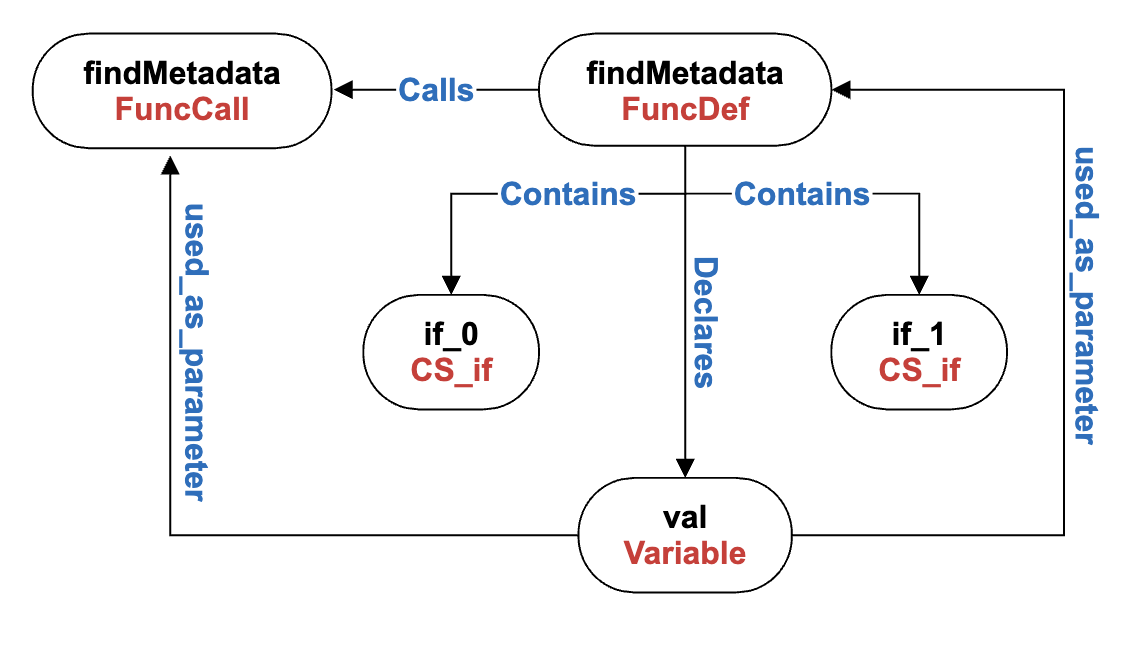
\includegraphics[width=0.6\textwidth]{graph_for_entry_9_in_db.png} 
    \caption{Graph generated from the code seen in Code Block \ref{lst:code_example}}  % The caption text
    \label{fig:graph_example}  % A label for referencing the figure in your document
\end{figure}

\subsubsection{Node Feature Matrix Generation}
Firstly, a node feature matrix, $X$, will need to be generated in order to capture node information. To capture semantic information for node identifiers (variable or function names), we utilized the popular natural-language-processing tool Word2Vec \cite{word2vec} to create vector embeddings from words. The model was trained on entire tokenized functions from the dataset. Vectors in $X$ were then generated containing: 
\begin{enumerate}
    \item A one-hot encoded vector $t_i \in {0, 1}^7$ representing the node type of node $i$. The vector contains a single 1 at the index corresponding to the node’s type (e.g., \texttt{FunctionCall}, \texttt{Variable}, etc.), and 0s elsewhere.
    \item An embedding vector $e_i \in \mathbb{R}^{100}$, computed as the average of the Word2Vec embeddings of the subtokens extracted from the node's name. If no subtokens are matched in the Word2Vec vocabulary, $e_i$ defaults to the zero vector.
\end{enumerate}
Thus, the vector $x_i \in X$ for node $v_i \in V$ is: $[t_i, e_i]^T$. 
The full node feature matrix \( X \in \mathbb{R}^{|V| \times 107} \) is defined as:

\[
X = 
\begin{bmatrix}
t_1 & t_2 & t_3 & \dots \\
e_1 & e_2 & e_3 & \dots
\end{bmatrix}
=
\begin{bmatrix}
x_1, x_2, \dots, x_{|V|}
\end{bmatrix}
\]

% Node Type Table
\begin{table}[h]
\centering
\begin{tabular}{ll}
\hline
\textbf{Node Type} & \textbf{Description} \\
\hline
\texttt{FunctionCall} & Represents a function call \\
\texttt{Variable} & A named variable in the code \\
\texttt{ControlStructure\_if} & An if-statement branch \\
\texttt{ControlStructure\_while} & A while-loop construct \\
\texttt{ControlStructure\_switch} & A switch-case block \\
\texttt{ControlStructure\_for} & A for-loop construct \\
\texttt{FunctionDefinition} & A function definition\\
\hline
\end{tabular}
\caption{Predefined node types used in graph construction.}
\label{tab:nodetypes}
\end{table}

\subsubsection{Edge Index and Edge Type Matrix Generation}
To construct the edge-related data for the GNN, we utilize two structures:

\begin{enumerate}
    \item The \textbf{edge index matrix} $E \in \mathbb{Z}^{2 \times |E|}$, which encodes the graph's edges. Each column represents a directed edge $(u, v)$, where $u$ and $v$ are node indices from the node feature matrix $X$. This is essentially an adjacency matrix compatible with PyTorch Geometric.
    \item The \textbf{edge attribute vector} $A \in \mathbb{Z}^{|E|}$, where each entry corresponds to an edge type (Table \ref{tab:edgetypes}) for the respective edge $e_i$.
\end{enumerate}
Given a graph $G = (V, E)$, we iterate over each edge $(u, v) \in E$ and extract its edge type (e.g., \texttt{calls}, \texttt{declares}, etc.). Each edge is mapped to an integer according to a pre-defined mapping. If an edge type is not recognized, it is assigned a value of $-1$ to be ignored during training. \\

Each graph $G$ is thus represented by three components: a node feature matrix $X$, the edge index matrix $E$, and the edge attribute vector $A$, which collectively define the input to the GNN model.

\begin{table}[h]
\centering
\begin{tabular}{lp{8cm}}
\hline
\textbf{Edge Type} & \textbf{Description} \\
\hline
\texttt{declares} & Indicates a declaration relationship. \\
\texttt{calls} & Represents a function call from one node to another. \\
\texttt{contains} & Denotes structural containment (e.g., a function contains a statement). \\
\texttt{used\_in\_condition} & Marks variables or expressions used in control conditions such as \texttt{if}, \texttt{while}, or \texttt{switch} statements. \\
\texttt{used\_as\_parameter} & Marks nodes that are passed as parameters to a function call. \\
\texttt{used\_in\_body} & Captures general usage of elements inside the body of a function or code block. \\
\hline
\end{tabular}
\caption{Predefined edge types used in graph construction.}
\label{tab:edgetypes}
\end{table}

\subsection{Architecture}
\subsubsection{The Convolution Layer}
Many existing graph neural network approaches to vulnerability detection have used aggregation techniques like graph convolution networks (GCNs) \cite{gcn}, graph attention networks (GATs) \cite{gat}, gated graph recurrent networks (GGRNs), and their variants. For this project, designed and tested three models, each of which using either GCNs, RGCNs, or GATs.
\paragraph{Graph Convolution Layer (GCN)}
\begin{description}
  \item[GCN \cite{gcn}:] Uses the propagation rule: 
  \[
  \mathbf{H}^{(l+1)} = \sigma\left( \tilde{\mathbf{D}}^{-\frac{1}{2}} \tilde{\mathbf{A}} \tilde{\mathbf{D}}^{-\frac{1}{2}} \mathbf{H}^{(l)} \mathbf{W}^{(l)} \right)
  \]
  where $\tilde{\mathbf{A}} = \mathbf{A} + \mathbf{I}_N$ is the adjacency matrix of the graph $G$ with added self-loops, and $\tilde{\mathbf{D}}_{ii} = \sum_j \tilde{\mathbf{A}}_{ij}$ is the corresponding degree matrix (containing the number of connected edges per node). $\mathbf{W}^{(l)}$ is the trainable weight matrix for layer $l$, and $\sigma(\cdot)$ is a nonlinear activation function like ReLU. $\mathbf{H}^{(l)}$ denotes the output node embeddings after layer $l$, with $\mathbf{H}^{(0)} = \mathbf{X}$, the initial input features.

  \item[GAT \cite{gat}:] Graph Attention Networks compute attention scores between nodes and their neighbors:
  \[
    \alpha_{ij} = \frac{\exp(\text{LeakyReLU}(\textbf{a}^T[\mathbf{W}h_i || \mathbf{W}h_j]))}{\sum_{k \in \mathcal{N}_i} \exp(\text{LeakyReLU}(\textbf{a}^T[\mathbf{W}h_i || \mathbf{W}h_k]))}
  \]
  where $\big\Vert$ represents the concatenation operation. $h_i$ represents the set of node features for node $i$. A shared linear transformation is applied to every node through the learnable weight matrix $\textbf{W}$. Additionally, a shared attention mechanism, $\textbf{a}$, is applied to every transformation, and is used to compute the importance of node $j$'s features on node $i$. $\mathcal{N}_i$ represents the set of neighbor nodes of node $i$ in the graph. $\alpha_{ij}$ represents the attention coefficient, representing the normalized importance of node $j$'s features on node $i$. Then, the result of feature aggregation, $h_i'$, is obtained through multi-head attention mechanisms as follows:
  \[
    h_{i}' = \big\Vert_{k=1}^K \sigma(\sum_{j \in \mathcal{N}_i} \alpha_{ij}^k \textbf{W}^k h_j)
  \]
  where $\alpha_{ij}^k$ are normalized attention coefficients computed at the $k^{th}$ attention mechanism and $\mathbf{W}^k$ is the linear transformation weight matrix for attention mechanism $k$.


  \item[RGCN \cite{rgcn}:] Relational Graph Convolution Networks extend GCNs to handle multiple edge types:
  \[
  \mathbf{h}_i^{(l+1)} = \sigma\left( \sum_{r \in \mathcal{R}} \sum_{j \in \mathcal{N}_i^r} \frac{1}{c_{i,r}} \mathbf{W}_r^{(l)} \mathbf{h}_j^{(l)} + \mathbf{W}_0^{(l)} \mathbf{h}_i^{(l)} \right)
  \]
  where $\mathcal{R}$ is the set of relation types, and $\mathcal{N}_i^r$ denotes the set of neighborhood indices to node $i$ of relation $r$. $\mathbf{W}_r^{(l)}$ is a learnable weight matrix specific to relation $r$. $c_{i, r}$ is a problem-specific normalization constant that can either be learned or chosen in advance. $\mathbf{W}_0^{(l)} \mathbf{h}_i^{(l)}$ is added to account for self-loop contributions.

\end{description}

\subsubsection{Model Flow}
Each of the three models follow a similar flow:
\begin{enumerate}
    \item The node features are passed through the respective graph convolution layers, followed by activation functions (ReLU) and dropout for regularization.
    \item Node features are aggregated using global mean pooling to generate graph-level embeddings.
    \item The graph-level features are concatenated with additional graph-level flags and passed through an multi-layer perceptron for the final classification.
\end{enumerate}

\subsection{Evaluation}
To assess the performance of our graph-based model, we aimed to answer the following questions: \\
\textbf{Q1: } How does our model compare to the state-of-the-art graph-based binary classification models? \\
\textbf{Q2: } Which of the convolution models provides the best performance? \\
\textbf{Q3: } What types of vulnerabilities does the model continuously fail to identify? \\
\textbf{Q4: } How does the model handle class imbalance? \\
\textbf{Q5: } What are the next steps needed to improve the performance of vulnerability detection via machine learning methods?

\subsubsection{Dataset preparation}
Many popular datasets exist for vulnerability detection; however, they all have a severe imbalance between vulnerable and non-vulnerable entries, with vulnerable entries being in the extreme minority. To that end, we chose to combine the \textit{PrimeVul} \cite{primevul}, \textit{BigVul} \cite{bigvul}, and \textit{DiverseVul} \cite{diversevul} datasets. Then, duplicate entries across datasets were removed, leaving a combined dataset with $29,867$ vulnerable entries and $506,084$ safe entries (Table \ref{tab:dataset_entries}). Safe entries were downsampled across the entire dataset. In the training dataset, vulnerable entries were randomly oversampled to achieve a 50/50 split between vulnerable and safe entries (Table \ref{tab:train-test-valid-split}). Entries in the dataset were then randomly shuffled. All of the GNN-based models were tested on the complete dataset, and the PrimeVul dataset.

\begin{table}[h]
 \centering
 \resizebox{\textwidth}{!}{ % Adjusts the table to the width of the text
 \begin{tabular}{|l|c|c|c|c|}
 \hline
 \textbf{Dataset} & \textbf{Total Entries} & \textbf{Percent Duplicates} & \textbf{Vulnerable Entries} & \textbf{Safe Entries} \\
 \hline
 \multicolumn{5}{|c|}{\textbf{Complete Dataset}} \\
 \hline
 Train & 354,258 & 44.00\% & 177,129 (50.00\%) & 177,129 (50.00\%) \\
 Test & 80,393 & 0.00\% & 4,480 (5.57\%) & 75,913 (94.43\%) \\
 Validation & 80,393 & 0.00\% & 4,480 (5.57\%) & 75,913 (94.43\%) \\
 \hline
 \multicolumn{5}{|c|}{\textbf{PrimeVul Dataset}} \\
 \hline
 Train & 8,406 & 41.67\% & 4,203 (50.00\%) & 4,203 (50.00\%) \\
 Test & 6,363 & 0.00\% & 900 (14.14\%) & 5,463 (85.86\%) \\
 Validation & 6,364 & 0.00\% & 901 (14.16\%) & 5,463 (85.84\%) \\
 \hline
 \end{tabular}
 }
 \caption{Datasets used for training, testing, and validation for Complete and PrimeVul datasets}
 \label{tab:train-test-valid-split}
\end{table}



\subsubsection{Results}
In the embedding layer, the dimension of Word2Vec for the initial node representation is 100. For the GCN, GAT, and RGCN layers, the dimension of hidden states was set to 128. Three convolution layers were used for all three convolution types. We use the Adam optimizer with a learning rate of $0.001$, and batch size of $128$. We additionally used an L2 regularization rate of $1 \times 10^{-5}$, and dropout of $0.3$ to minimize overfitting. Each model was evaluated over 25 epochs. The decision threshold was adjusted based on Youden's J statistic from the ROC curve, aiming to balance vulnerable samples and false positives. All models were tested after training using the test dataset, while during training, they were tested using the validation dataset after each epoch. See Table \ref{tab:performance-metrics} for results. 
\paragraph{GCN:} The model using the GCN convolution achieved very low precision, indicating a high number of misclassifications of safe samples as vulnerable. However, it demonstrated high recall, reflecting a strong ability to identify vulnerable samples. This is particularly valuable in vulnerability detection, where false negatives are more detrimental than false positives. Despite this, the model showed unstable validation accuracy compared to the more consistent training accuracy (Figure \ref{fig:gcn_acc}).

\paragraph{GAT:} The model using the GAT convolution achieved moderate precision, indicating a relatively low rate of misclassify safe samples as vulnerable. While its recall is also moderate, it reflects a balanced ability to identify vulnerable samples. Additionally, the model achieved precision accuracy closer to train accuracy, indicating less overfitting and better generalization (Figure \ref{fig:gat_acc}).

\paragraph{RGCN:} The model utilizing the RGCN convolution achieved a precision of 0.177—the highest among all architectures—highlighting its strong ability to minimize false positives. In terms of recall, the RGCN reached 0.639, which, while slightly lower than the values observed in GAT and GCN-based models, still reflects a strong ability to capture true positives. Additionally, the RGCN exhibited relatively stable and high validation accuracy throughout training, consistently ranging between $80$\% and $85$\% (Figure \ref{fig:rgcn_acc}).

\paragraph{Devign:} The state-of-the-art Devign model exhibited relatively high precision, indicating that it is conservative in predicting vulnerabilities and avoids misclassifying safe samples as vulnerable. However, its recall was significantly lower, meaning it misses a substantial number of true positives. Devign also demonstrated the lowest accuracy of all models at $43.6$\%.

\begin{table}[h]
    \centering
    \begin{tabular}{|l|c|c|c|c|c|}
        \hline
        \textbf{Model} & Accuracy & Precision & Recall & F1 Score & AUC \\
        \hline
        \multicolumn{6}{|c|}{\textbf{Complete Dataset}} \\
        \hline
        \textbf{GCN}  & 0.6084  & 0.1045  & 0.7960  & 0.1847  & 0.766 \\
        \textbf{GAT}  & 0.7545  & 0.1373  & 0.6444  & 0.2264  & 0.766 \\
        \textbf{RGCN} & 0.8142  & 0.1770  & 0.6393  & 0.2772  & 0.799 \\
        \textbf{Devign} & 0.4360 & 0.4470 & 0.4040 & 0.4240 & 0.453 \\
        \hline
        \multicolumn{6}{|c|}{\textbf{PrimeVul Dataset}} \\
        \hline
        \textbf{RGCN}  & 0.3929  & 0.1821  & 0.9433  & 0.3053  & 0.742 \\
        \textbf{GCN}   & 0.3442  & 0.1654  & 0.8989  & 0.2794  & 0.669 \\
        \textbf{GAT}   & 0.3539  & 0.1677  & 0.9000  & 0.2827  & 0.676 \\
        \textbf{Devign} & 0.4850 & 0.5000 & 0.4810 & 0.4900 & 0.486 \\
        \hline
    \end{tabular}
    \caption{ML Stats for Complete and PrimeVul Datasets}
    \label{tab:performance-metrics}
\end{table}

\begin{figure}[h]
    \centering
    \begin{minipage}{0.32\textwidth}
        \centering
        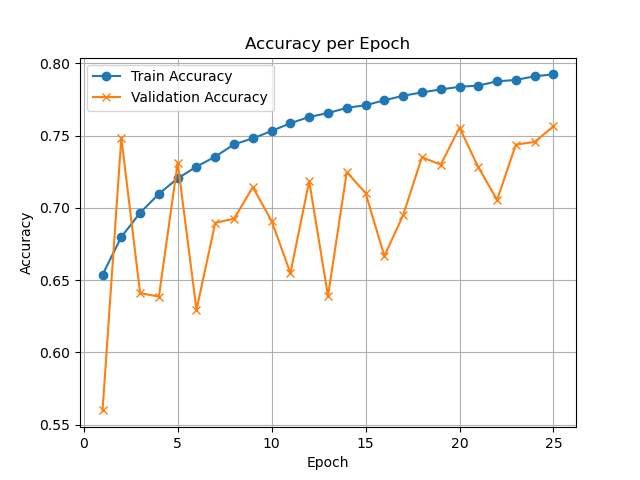
\includegraphics[width=\textwidth]{gat_acc.png}
        \caption{GAT Accuracy (Complete)}
        \label{fig:gat_acc}
    \end{minipage}
    \hfill
    \begin{minipage}{0.32\textwidth}
        \centering
        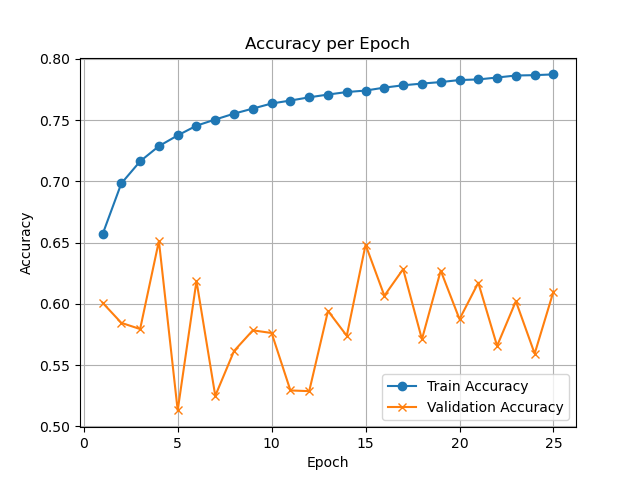
\includegraphics[width=\textwidth]{gcn_acc.png}
        \caption{GCN Accuracy (Complete)}
        \label{fig:gcn_acc}
    \end{minipage}
    \hfill
    \begin{minipage}{0.32\textwidth}
        \centering
        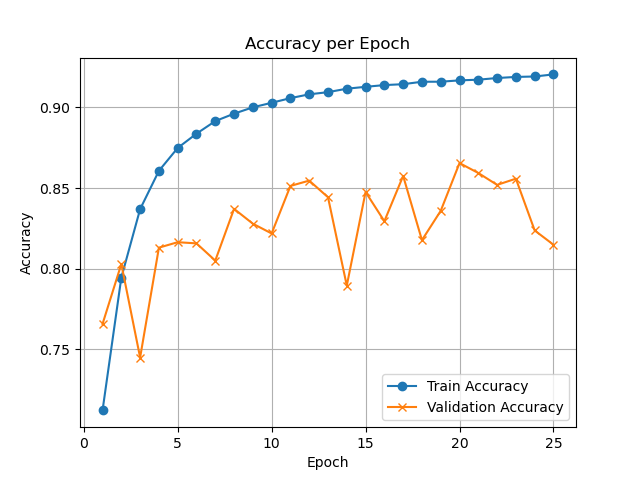
\includegraphics[width=\textwidth]{rgcn_acc.png}
        \caption{RGCN Accuracy (Complete)}
        \label{fig:rgcn_acc}
    \end{minipage}
    
    \vspace{0.5cm} % Adds a little space between rows
    
    \begin{minipage}{0.32\textwidth}
        \centering
        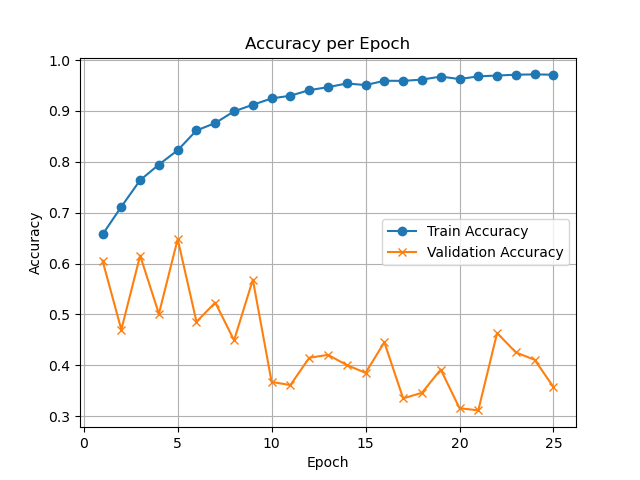
\includegraphics[width=\textwidth]{pv_gat_acc.png}
        \caption{GAT Accuracy (PrimeVul)}
        \label{fig:pv_gat_acc}
    \end{minipage}
    \hfill
    \begin{minipage}{0.32\textwidth}
        \centering
        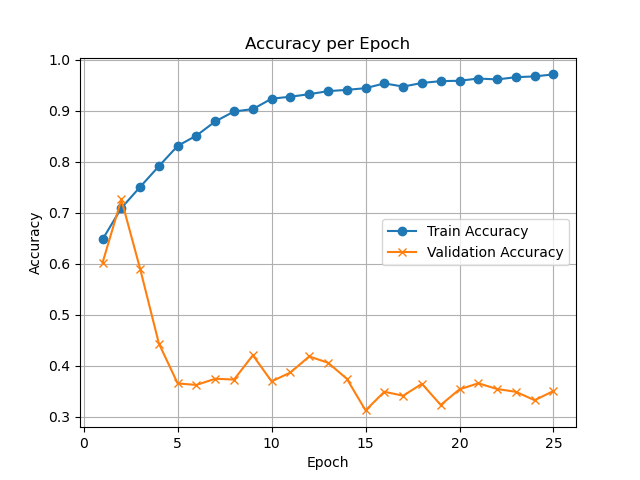
\includegraphics[width=\textwidth]{pv_gcn_acc.png}
        \caption{GCN Accuracy (PrimeVul)}
        \label{fig:pv_gcn_acc}
    \end{minipage}
    \hfill
    \begin{minipage}{0.32\textwidth}
        \centering
        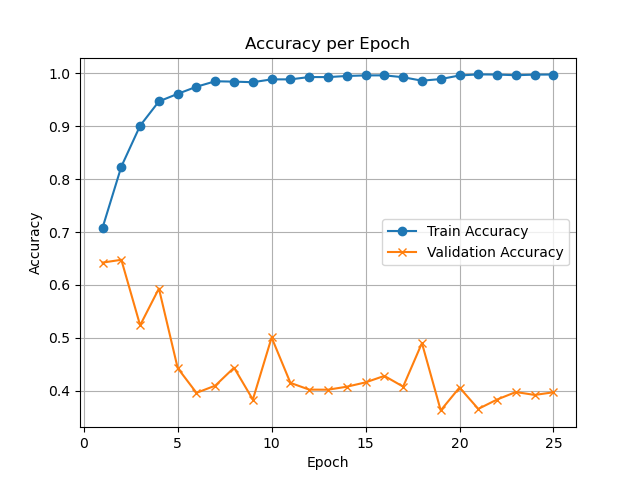
\includegraphics[width=\textwidth]{pv_rgcn_acc.png}
        \caption{RGCN Accuracy (PrimeVul)}
        \label{fig:pv_rgcn_acc}
    \end{minipage}

    \caption{Accuracy Curves for GAT, GCN, and RGCN across Complete and PrimeVul Datasets}
    \label{fig:acc_curves}
\end{figure}

\paragraph{Performance on specific vulnerabilities:}\label{sec:performance-on-vulns} Based on results from the RGCN model, the model classified the following vulnerabilities well: authentication bypass, improper initialization, and missing encryption, achieving $100$\% detection rates on all three (Table \ref{tab:vulnerabilities}). The model fails to fully identify the following vulnerabilities: resource management error, information exposure, race condition, numeric error, and inadequate access controls, only achieving between $60$-$70$\% detection on these vulnerabilities (Table \ref{tab:vulnerabilities}).

\begin{table}[h]
    \centering
    \resizebox{\textwidth}{!}{
    \begin{tabular}{|l|c|c|c|}
        \hline
        \textbf{Vulnerability Type} & \textbf{CWE} & \textbf{Sample Size} & \textbf{Detection Rate (\%)} \\ 
        \hline
        \multicolumn{4}{|c|}{\textbf{Best Performing}} \\
        \hline
        Authentication Bypass & CWE-290 & 21 & 100.00\% \\
        Improper Initialization & CWE-665 & 15 & 100.00\% \\
        Missing Encryption & CWE-311 & 52 & 100.00\% \\
        \hline
        \multicolumn{4}{|c|}{\textbf{Worst Performing}} \\
        \hline
        Resource Management Error & CWE-399 & 4218 & 63.00\% \\
        Information Exposure & CWE-200 & 4865 & 65.60\% \\
        Race Condition & CWE-362 & 2755 & 69.30\% \\
        Numeric Error & CWE-189 & 4093 & 65.30\% \\
        Inadequate Access Controls & CWE-772 & 996 & 61.00\% \\
        \hline
    \end{tabular}
}
\caption{Comparison of Best and Worst Performing Vulnerabilities}
\label{tab:vulnerabilities}
\end{table}

\subsubsection{Discussion}
The results indicate that, while Graph Neural Networks (GNNs) show potential in vulnerability detection, there remains significant room for improvement, especially when considering the low F1 scores observed across all models. The trade-offs between precision, recall, and F1 score highlight the challenges of achieving a balanced and effective model for vulnerability detection.

\paragraph{Comparison Between Datasets:} 
A notable comparison is between the performance on the Complete dataset and the PrimeVul dataset. While the models performed relatively well on the Complete dataset, achieving an accuracy of around 60-80\% for GCN, GAT, and RGCN, the performance on the PrimeVul dataset alone was much lower. Though the F1 scores are misleadingly higher (Table \ref{tab:performance-metrics}), the  accuracy is extremely low. Additionally, during training, the validation accuracy plummets, indicating the PrimeVul dataset alone does not have enough information to allow the model to generalize. Thus, all models were trained on the combined dataset.

\paragraph{Precision vs Recall}
The GCN model demonstrated high recall but very low precision, meaning that while it was able to identify many of the vulnerable samples, it frequently misclassified safe samples as vulnerable. While it is important in vulnerability detection to minimize false negatives (i.e. avoid misclassifying vulnerable code as safe), the low F1 score, precision, and accuracy indicates the model is not generalizing well on the data.

In contrast, the GAT model displayed more stable validation accuracy, suggesting that it has better generalization capabilities. The model also demonstrates higher accuracy, precision, recall, and F1, indicating the GAT convolution is better at learning vulnerability patterns from the graph. However, there is still a lot of room for improvement.

The RGCN model performed the best overall, with the highest F1 score and validation accuracy. Though it has lower recall as compared to the GAT and GCN, it demonstrates the best balance between precision and recall. Additionally, its stable and high validation accuracy indicates a better ability to generalize insights from the train data on the validation dataset. Overall, the high accuracy and F1 achieved using the RGCN convolution make it the most reliable for vulnerability detection in this study. However, its slightly lower recall compared to the GCN suggests that further improvements can be made to maximize its sensitivity to vulnerabilities.

\paragraph{Most Frequently Misclassified Vulnerabilities:} While the model is good at detecting certain vulnerabilities (Table \ref{tab:vulnerabilities}), the sample sizes for these vulnerabilities is fairly low and inconclusive. The worst performing vulnerabilities, including resource management error, information exposure, race condition, numeric error, and inadequate access controls, involve complex patterns that the model may struggle to identify. Though a detection rate of $60$-$70$\% is not ideal, it is still better than a random guess. 

\paragraph{Devign}
The state-of-the-art Devign model utilizes word embeddings (with Word2Vec) with graph-based features, similarly to our model. Devign uses Joern \cite{joern}, a pre-existing tool to generate complex code property graphs, as compared to our fairly simple graph representations. Devign also utilizes Gated Graph Recurrent Networks \cite{ggrn}, where we use GCNs, GATs, and RGCNs. Devign showed relatively high precision, meaning it is cautious in predicting vulnerabilities and avoids misclassifying safe samples as vulnerable. However, its low recall indicates that it misses a significant portion of true vulnerabilities. The model also demonstrated the lowest accuracy and AUC among all models, which indicates that Devign struggles to generalize well to the validation dataset. The combination of low recall and accuracy points to significant limitations in its ability to perform well in vulnerability detection on the current dataset.

\paragraph{Conclusion}
The low F1 scores across all architectures suggest that there is still much to be done to improve the models' performance, particularly in terms of increasing recall while maintaining precision. A possible approach to achieving this goal would be to improve graph expression of data. One popular graph generation tool is Joern \cite{joern}, which generates more complex code property graphs (CPGs). Along with this, further exploration of feature engineering could help create better code context, helping the model detect complex vulnerabilities easier. Additionally, further work will need to be done to find vulnerable samples, as the massive class imbalance in the dataset has limited the performance of the model.

Overall, when comparing our model with the state-of-the-art model Devign, it is clear we have made some improvements toward vulnerability detection. However, more work will need to be done in order to detect complex vulnerabilities more reliably.

\clearpage
\bibliographystyle{plainnat}
\bibliography{sources}
\end{document}
